\section{Challenges in non-commute travel demand forecast}

Estimating trip attraction is a crucial topic of the transport planning academic literature and profession, constituting an integral component of the demand forecast framework, termed the Four-Step Model (FSM), which has been in ubiquitous use since the 1950s \citep{TravelForecastingResource}. More specifically, the FSM begins with the Trip Generation step, where the number of trips generated by each traffic analysis zone is estimated, and Trip Distribution allocates these trips to their destination zones before proceeding to mode choice determination and route assignment. Planners accomplish the task of Trip Distribution using a variety of spatial interaction models, most prominent among which is the classic \textit{Gravity Model} and its derivatives inspired by Newton's law of universal gravitation \citep{erlanderGravityModelTransportation1990}. Originally formulated to estimate flows among cities in a region, it has been adapted to intraurban mobility and suggests that the number of trips between two locations is proportional to the difference in \textit{mass} of each location (Origin and Destination) and inversely proportional to the distance between them. 

\begin{figure}[h]
    \centering
    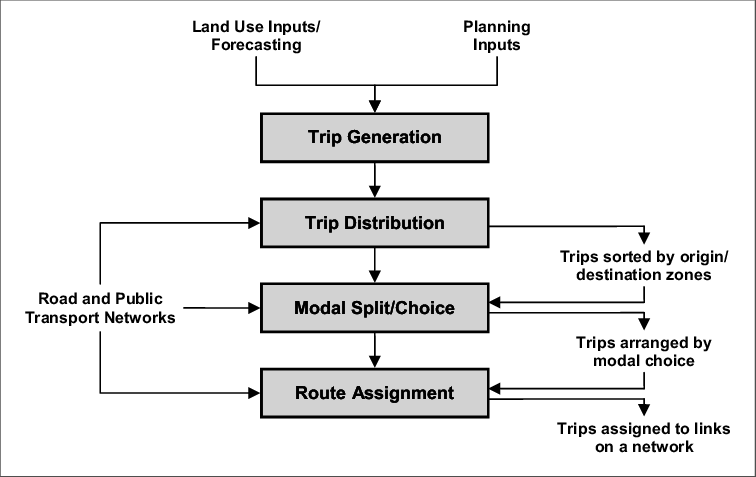
\includegraphics{fsm.png}
    \caption{Traditional four-step transport model (FSM)}
    \captionsetup{aboveskip=0pt,font=it}
    \caption*{Source: \cite{evansClothingEmperorTransport2007}}
    \label{fig:fsm}
\end{figure}

However, it is worth noting that the definition of \textit{mass} in any gravity-based spatial interaction model has seen many interpretations and experimentations, depending on the types of travel demand of research interest. For example, a spatial interaction model for commuting trip forecasts may consider the emissivity of residential areas as origins and the attractiveness of employment centres as destinations. In fact, the estimation of trip attraction in transport planning literature has predominantly revolved around commutes (i.e., primary travel demand) from residential zones to zones where employment centres or education institutions are located. On the one hand, this choice is a practical one first and foremost, as commuting trips represent a large share of regular intracity mobility flows, whose high volume within short peak periods has important implications on road capacity management or public transit operations, among others. Due to its importance, the calibration of the spatial interaction model for commuting flows is further aided by nationwide flow datasets, such as that present in the UK Census Data\footnote{An interactive visualisation of the UK Census 2021 origin-destination data can be found at \url{https://www.ons.gov.uk/visualisations/censusorigindestination/}}, which provides detailed and explicit Origin-Destination data to serve as ground truth. In the absence of this declared data, researchers have also turned to spatial features to calibrate commute trip distribution, as explored by \cite{yangLimitsPredictabilityCommuting2014}.

On the other hand, a plethora of potential trips generated for other purposes is often underresearched, partially due to the complexity of non-commute trip purpose identification, classification and quantification: Non-commute trips can be defined as trips that are not carried out to fulfil time-bound and regular work or education obligations and can include trips for shopping, leisure, and social activities. Therefore, as opposed to commuting trips, Non-commute trips are highly irregular both spatially and temporally, i.e., they can vary in terms of distance, duration, and mode of transport from one to another, even for the same destination between different days. Nevertheless, Non-commute trips are an important component of urban travel behaviour and can have a significant impact on the overall transportation system. Advances in the field have brought about improvements to methodologies such as travel diary surveys\footnote{An example of these is the UK National Travel Survey, accessible at \url{https://www.gov.uk/government/collections/national-travel-survey-statistics}}, which collect data on personal and household travel behaviour, including Non-commute trips, to allow for comprehensive planning. By design, however, they are limited in scale and generalisability.

Overall, this reveals a gap in our understanding of the comprehensive travel behaviour of city dwellers on an aggregate scale. With the number of trips for shopping, leisure, and social activities increasing in recent years and the number of work-related trips decreasing as flexible work arrangements become more prevalent \citep{wohnerWorkFlexiblyTravel2022}, with recognised health benefits to workers \citep{macleodCommutingWorkPostpandemic2022}, it is important to understand the factors that influence non-commute trip attraction and to incorporate them into transport planning models.  

In the scope of this research, we hypothesise that a given urban area's non-commute trip attracting \textit{mass} is associated with the built environments, which include their amenity and public transport accessibility profiles. 

\section{Urban amenities as attractors}

\cite{cerveroTravelDemand3Ds1997} was one of the foundational works to provide an econometric estimation of how three groups of factors pertaining to the built environments---namely Density, Diversity and Design---are associated with travel demand to a traffic analysis zone for different purposes (work/non-work) and with different mode choices (private vehicles/public transport). This study is novel for demonstrating that changes in the built environment—such as density, diversity, and walkability have a tangible impact on travel behaviour, which supports the idea that designing more compact, mixed-use, pedestrian-friendly neighbourhoods can significantly influence how people choose to travel. The components of density and diversity refer to the number and the variety of destinations available in a given area, respectively, while the design component refers to the physical layout of the area, including the presence of sidewalks, bike lanes, and other pedestrian-friendly infrastructure. It is worth noting that the study considered the distance as a control impedance factor---adhering to the classic Gravity Model paradigm---and did not investigate how these factors may interact with each other.

There have been many recent attempts to link the presence of urban amenities to trip attraction and calibrate how we define urban attractors. Beyond pure correlation observed between the density of points of interest (POIs) in a region and intensity of trips made to a given area \citep{melikovCharacterizingUrbanMobility2021}, the typology of the POIs differs between urban clusters that see distinct patterns of inflow trips made. For example, after \citet{aaqibjavedEstimationTripAttraction2020} have clustered urban areas in one city into Global (e.g., airports), Downtown (d.g., central business district) and Residential attractors based on the volume, spatial dispersion and distance of the trips made using O-D data from mobile phone, they found that the differences in the types of POIs in each of these clusters were also statistically significant. The typology of amenity POIs explored in this study included not only Retail, as is common when thinking about non-commute trips, but also hospitals, public services, restaurants, religious institutions, and other categories. This suggests that the type of urban amenities available in an area can influence the volume of trips made to that area and that different types of amenities may attract different types of trip purposes.

\section{Transport accessibility as attractors}

If the density and diversity of amenities were the only explanatory factors for non-commute trip demand, it would be tempting to conclude that the local configuration of destination points of interest is the sole determinant of why people go to one place and not another for their diverse needs. In reality, neighbourhoods do not exist in a vacuum but are intricately connected to one another by the transportation network. In simple terms, the consideration of distance as friction in the classic Gravity Model attests to the fact that the more accessible a destination is, the more likely it is to attract travel demand, especially trips with higher elasticity of choice such as non-commute (i.e., trips made to a specific destination not based on obligation, but mainly out of convenience). 
Public transport accessibility has been shown to contribute to the growth of intercity importance of certain areas as opposed to others and preserve travel demand variability over time \citep{zhongMeasuringVariabilityMobility2015}, which means that it reinforces the prominence of well-connected areas as urban attractors, presumably with similar density and diversity of destination points of interest. 

\cite{jayasingheApplicationDevelopingCountries2017} went one step further to purport that the network centrality property of an urban area is enough to predict travel demand to a high degree of accuracy without the need to consider other attractors such as employment centres and amenities, thanks to its tight correlation. More specifically, the study looked at four centrality measures: Connectivity, Choice, Global Integration and Local Integration, which are analogous to the concept of degree centrality, betweenness centrality, closeness centrality, and closeness centrality in a confined radius, respectively. Among them, Global Integration (closeness centrality) was found to be the most significant predictor, suggesting that the role of the transport network in shaping urban travel demand at the aggregate scale is paramount, perhaps just as important as socio-economic factors \citep{converyDeterminantsTransportMode2019}

\section{Public transport and the walkable city}

Walkability contributes to the quality of life in cities. The 15-minute city is one of the most recent urban planning concepts that has gained traction in recent years. The idea is to create more sustainable and resilient cities by reducing the need for long commutes and promoting active modes of transport such as walking and cycling. A resident who lives in a neighbourhood that has all the amenities they need within a 15-minute walk or cycle can ideally reduce their reliance on cars and public transport to a minimum. However, this does not mean that the role of public transport is diminished within the 15-minute city vision. On the contrary, public transport is an essential component of a sustainable system, which provides an efficient and affordable way for people to travel longer distances, effectively agglomerating a larger urban system made up of ideally 15-minute cities. In other words, public transport is the backbone of the 15-minute city, connecting neighbourhoods and enabling people to travel further than they can on foot or by bike. This, in turn, has multiple implications for the local communities:

\begin{itemize}
    \item From the lens of urban planning and traffic management, the higher the volume of public transport trips made to an area, the higher the amount of pedestrian traffic it receives on top of the local population who patronises their local amenities. Understanding the trip attraction factors can help prioritise investments in public transport capacity planning, pedestrian or cycling infrastructures and services for these individuals, which can lead to a virtuous cycle of increased active travel and reduced car dependency.
    \item From the lens of fomenting local economies, increased pedestrian traffic injected by public transport can also be seen as an additional source of footfall, which is invaluable for businesses with storefronts. Findings on the economic benefits of walking and cycling done by Transport for London\footnote{https://tfl.gov.uk/corporate/publications-and-reports/economic-benefits-of-walking-and-cycling} showed that retail rents increased by 7\%, and office space rents increased by 4\% in areas that encouraged non-motorised access, suggesting that the street improvements translated into much more desirable spaces.
\end{itemize}

It is also worth mentioning that footfall estimation itself is a prolific field of research within retail analytics, which counts on a variety of technologies such as WiFi tracking, video analytics, and mobile phone data to estimate the number of people who pass by a given location. The insights derived from footfall data can be used to inform decisions on store location, opening hours, staffing levels, and marketing strategies, among others. Uncovering patterns of public transport trip attraction, which in turn is an indicator of pedestrian influx, could be used to complement footfall data and provide a more comprehensive understanding of the factors that influence the number of people in a given area.

\section{Explainable Artificial Intelligence for spatial systems}

Up to this point, our visited literature has shown that both urban amenities and transport accessibility are important factors in determining the attractiveness of an area to non-commute trips, albeit in isolation. In reality, the interaction between these two factors has not been well studied in conjunction. It is possible that the dense presence of diverse urban amenities is brought about by preexisting favourable transport accessibility or vice versa. In the interest of addressing the research questions, we are presented with a dilemma of interpretability versus prediction accuracy in the choice of modelling techniques.

Econometric methods, commonly used in policy analysis, can help us quantify and interpret the relationship between the dependent variables and independent variables in the form of explicit coefficients. However, even spatially aware methods such as Spatial Lag Model (SLM) or Geographically Weighted Regression (GWR) are limited in their linear assumptions of linearity, issues with multicollinearity, and thus may fail at attaining high prediction accuracy \citep{wheelerMulticollinearityCorrelationLocal2005}.

In the meantime, machine learning methods have gained popularity in the field of urban mobility research due to their ability to capture complex, non-linear relationships between spatial features with high prediction accuracy. However, the lack of interpretability of machine learning models has been a major drawback, especially in the context of urban planning, where the ability to understand the underlying factors that drive the model's predictions is crucial for decision-making. Among many opportunities to develop Machine Learning explanation techniques for causal inference in urban mobility is the need to evaluate causal effects of input features and derive actionable insights \citep{xinVisionPaperCausal2022}.

To address the interpretability challenge, local interpretation methods like SHAP (SHapley Additive exPlanations)---a method based on cooperative game theory based on the seminal work by \cite{lundbergUnifiedApproachInterpreting2017a}---to provide detailed attributions of input features to individual predictions made. Its introduction contributed to the growing body of literature on interpretable machine learning with spatial systems for regression with XGBoost \citep{liExtractingSpatialEffects2022} or classification with Light GBM \citep{louhichiShapleyValuesExplaining2023}. One of the most notable recent examples of SHAP for urban mobility in action was the development of the Deep Gravity Model introduced by \cite{siminiDeepGravityModel2021}, which used SHAP to explain the predictions of a deep learning model for spatial interaction and how the model's predictions were influenced by the input spatial features such as land-use mix, points of interest in the origin and destination zones. 

As we approach this research with an eye on accurately modelling the real-world phenomenon and explaining the contributing factors, instead of GWR or SLM, we will use a machine learning model to predict non-commute trip attraction in urban areas and then leverage SHAP to explain the predictions in an attempt to quantify the relative importance and contribution of urban amenities and transport accessibility. The detailed methodology will be discussed in the next chapter.

\section{A remark on the use of open data}

Many recent advances in the field of urban mobility research have been made possible by the availability of proprietary datasets owned by private companies, such as mobile phone data, GPS data, and social media data. Although the high data granularity have opened doors to new research opportunities and development of new advanced techniques, its use also races concerns about data privacy, data ownership, and data sharing. Moreover, it heightens the barrier to entry for independent researchers who would like to replicate the studies for their respective cities or regions. In contrast, open data not only democratises independent and participatory research in the public interest, but also breaks down many reproducibility barriers when applying established methodologies to other localities \citep{yadavRoleOpenData2017}.

On one side, we have readily available open datasets maintained by local or federal government agencies in many countries, which in the case of London are the UK Census 2021 Data\footnote{https://www.nomisweb.co.uk/sources/census\_2021\_bulk} and Transport for London's GIS Open Data Hub\footnote{https://gis-tfl.opendata.arcgis.com/}. On the other, we have global platforms like \textbf{OpenStreetMap} and \textbf{Overture Maps Foundation} that provide a wealth of spatial data for cities around the world.

In this research, adhering to the spirit of openness and future reproducibility across different urban contexts, the datasets used will be entirely sourced from open data hubs and platforms with associated analysis scripts published to GitHub.
 